

\tikzset{every picture/.style={line width=0.75pt}} %set default line width to 0.75pt        

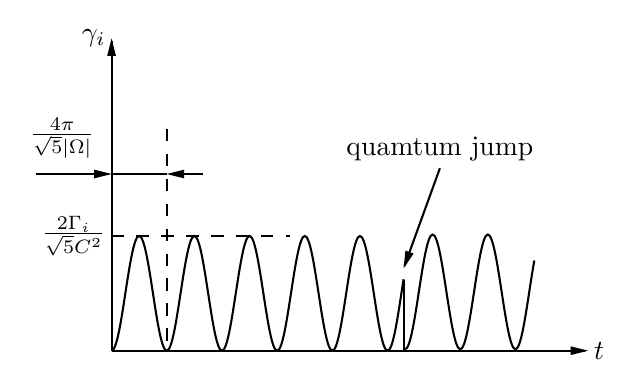
\begin{tikzpicture}[x=0.75pt,y=0.75pt,yscale=-0.7,xscale=0.7]
%uncomment if require: \path (0,300); %set diagram left start at 0, and has height of 300

%Straight Lines [id:da11432866530238495] 
\draw    (127,260) -- (453,260) ;
\draw [shift={(455,260)}, rotate = 180] [fill={rgb, 255:red, 0; green, 0; blue, 0 }  ][line width=0.08]  [draw opacity=0] (12,-3) -- (0,0) -- (12,3) -- cycle    ;
%Straight Lines [id:da5962017011774512] 
\draw    (127,260) -- (127,47.06) ;
\draw [shift={(127,45.06)}, rotate = 90] [fill={rgb, 255:red, 0; green, 0; blue, 0 }  ][line width=0.08]  [draw opacity=0] (12,-3) -- (0,0) -- (12,3) -- cycle    ;
%Shape: Wave [id:dp033712095240970186] 
\draw   (127,260) .. controls (130.44,260) and (133.4,240.75) .. (136.5,220.53) .. controls (139.6,200.31) and (142.56,181.06) .. (146,181.06) .. controls (149.44,181.06) and (152.4,200.31) .. (155.5,220.53) .. controls (158.6,240.75) and (161.56,260) .. (165,260) .. controls (168.44,260) and (171.4,240.75) .. (174.5,220.53) .. controls (177.6,200.31) and (180.56,181.06) .. (184,181.06) .. controls (187.44,181.06) and (190.4,200.31) .. (193.5,220.53) .. controls (196.6,240.75) and (199.56,260) .. (203,260) .. controls (206.44,260) and (209.4,240.75) .. (212.5,220.53) .. controls (215.6,200.31) and (218.56,181.06) .. (222,181.06) .. controls (225.44,181.06) and (228.4,200.31) .. (231.5,220.53) .. controls (234.6,240.75) and (237.56,260) .. (241,260) .. controls (244.44,260) and (247.4,240.75) .. (250.5,220.53) .. controls (253.6,200.31) and (256.56,181.06) .. (260,181.06) .. controls (263.44,181.06) and (266.4,200.31) .. (269.5,220.53) .. controls (272.6,240.75) and (275.56,260) .. (279,260) .. controls (282.44,260) and (285.4,240.75) .. (288.5,220.53) .. controls (291.6,200.31) and (294.56,181.06) .. (298,181.06) .. controls (301.44,181.06) and (304.4,200.31) .. (307.5,220.53) .. controls (310.6,240.75) and (313.56,260) .. (317,260) .. controls (320.44,260) and (323.4,240.75) .. (326.5,220.53) .. controls (327,217.25) and (327.5,214) .. (328,210.84) ;
%Straight Lines [id:da2086461360603018] 
\draw    (328,211.4) -- (328,260.23) ;
%Straight Lines [id:da25403249150794016] 
\draw  [dash pattern={on 4.5pt off 4.5pt}]  (165,107.4) -- (165,261.4) ;
%Straight Lines [id:da03200480378729842] 
\draw    (127,138.4) -- (165,138.4) ;
%Straight Lines [id:da6296287663686768] 
\draw    (353,134.4) -- (328.68,201.52) ;
\draw [shift={(328,203.4)}, rotate = 289.92] [fill={rgb, 255:red, 0; green, 0; blue, 0 }  ][line width=0.08]  [draw opacity=0] (12,-3) -- (0,0) -- (12,3) -- cycle    ;
%Straight Lines [id:da6999365213295103] 
\draw  [dash pattern={on 4.5pt off 4.5pt}]  (127,181) -- (250,181) ;
%Straight Lines [id:da16313341403336534] 
\draw    (75,138.4) -- (125,138.4) ;
\draw [shift={(127,138.4)}, rotate = 180] [fill={rgb, 255:red, 0; green, 0; blue, 0 }  ][line width=0.08]  [draw opacity=0] (12,-3) -- (0,0) -- (12,3) -- cycle    ;
%Straight Lines [id:da11854401822498306] 
\draw    (167,138.4) -- (190,138.4) ;
\draw [shift={(165,138.4)}, rotate = 0] [fill={rgb, 255:red, 0; green, 0; blue, 0 }  ][line width=0.08]  [draw opacity=0] (12,-3) -- (0,0) -- (12,3) -- cycle    ;
%Shape: Wave [id:dp6841801359876702] 
\draw   (329,259) .. controls (332.44,259) and (335.4,239.75) .. (338.5,219.53) .. controls (341.6,199.31) and (344.56,180.06) .. (348,180.06) .. controls (351.44,180.06) and (354.4,199.31) .. (357.5,219.53) .. controls (360.6,239.75) and (363.56,259) .. (367,259) .. controls (370.44,259) and (373.4,239.75) .. (376.5,219.53) .. controls (379.6,199.31) and (382.56,180.06) .. (386,180.06) .. controls (389.44,180.06) and (392.4,199.31) .. (395.5,219.53) .. controls (398.6,239.75) and (401.56,259) .. (405,259) .. controls (408.44,259) and (411.4,239.75) .. (414.5,219.53) .. controls (415.67,211.86) and (416.83,204.34) .. (418,197.94) ;

% Text Node
\draw (125,45.06) node [anchor=east] [inner sep=0.75pt]    {$\gamma _{i}$};
% Text Node
\draw (457,260) node [anchor=west] [inner sep=0.75pt]    {$t$};
% Text Node
\draw (93,130) node [anchor=south] [inner sep=0.75pt]    {$\frac{4\pi }{\sqrt{5} |\Omega |}$};
% Text Node
\draw (353,131.4) node [anchor=south] [inner sep=0.75pt]   [align=left] {quamtum jump};
% Text Node
\draw (125,181) node [anchor=east] [inner sep=0.75pt]    {$\frac{2\Gamma _{i}}{\sqrt{5} C^{2}}$};


\end{tikzpicture}
